%=======================================================
\section{Heterogeneity Dimensions}
\label{ssec:dimensions}
%=======================================================


The set of \acp{DT} belonging to the same ecosystem may be \emph{heterogeneous} for various reasons.
To better characterize this heterogeneity, we extract and analyze a set of orthogonal dimensions along which \acp{DT} may differ.

\Cref{tab:heterogeneity} briefly reports the dimensions we identified through an analysis of the relevant literature on \acp{DTE}.
We find that \acp{DTE} are usually envisioned in contexts that either involve multiple stakeholders (\emph{organization dimension}) and a diverse set of assets (\emph{domain dimension}) that may require different techniques to be described effectively (\emph{modeling dimension}).
Furthermore, as highlighted in \Cref{ssec:dt-background}, \acp{DT} are employed for a variety of use cases, ranging from monitoring to simulation and forecasting (\emph{purpose dimension}).

As an additional factor of complexity, different stakeholders may be interested in different views of the same \ac{PA}, ending up independently developing multiple \acp{DT} to fulfill distinct business goals~\cite{minerva2020dtiot}.
%
Ecosystems can then either serve a unifying purpose, connecting different views cof the same \ac{PA}, or exist in parallel to serve specific perspectives of the same domain.

All these factors naturally result in technological fragmentation (\emph{technology dimension}), which is particularly evident in the current \ac{DT} technology landscape.
%
While many commercial solutions remain focused on specific application domains~\cite{Damjanovic-Behrendt_Behrendt_2019}, the \ac{DT} community has witnessed the rise of both commercial and open-source technologies with a more general-purpose vocation.
%
Representative examples that we consider for our prototype \acp{DTE} can be found in major industries, such as Microsoft's Azure Digital Twins\footnote{\url{https://azure.microsoft.com/en-us/products/digital-twins}}, open-source solutions such as Eclipse Ditto\footnote{\url{https://eclipse.dev/ditto/index.html}} and independent efforts from the academic community such as the White Label Digital Twin Framework\footnote{\url{https://wldt.github.io}}~\cite{picone2021wldt}.

We conclude that, due to its multi-dimensional nature, heterogeneity should be regarded as an inherent source of complexity in \acp{DTE}.
We suggest that an analysis of such heterogeneity along the identified dimensions can guide architectural decisions for implementing the \ac{DTE}.


 \note{table}
% \begin{table*}[t]
%     \centering
%     \renewcommand{\arraystretch}{1.1}
%     \begin{tabular}{p{2.5cm}|p{\dimexpr\textwidth-3.5cm\relax}}
%     \toprule
%     \midrule
%     \textbf{Heterogeneity \newline Dimension} & \textbf{Description} \\
%     \hline
%     \hline
%     Organization &
%     \acp{DTE} may digitalize large-scale contexts involving \acp{PA} that belong to different stakeholders and organizations that may need to collaborate~\cite{tripathi2024infsof}
%     \\
%     \hline
%     Domain & 
%     Large \acp{DTE} may include assets from different application domains and hence require the integration of different domain vocabularies such as in the case of a smart city ecosystem that may span across the energy, mobility, ecology, and financial domains~\cite{deng2021systematic,del2024virtual}
%     \\
%     \hline
%     Purpose &
%     The \ac{DT} paradigm is employed for a variety of purposes~\cite{bulter2018geminiprinciples} leading to very different \acp{DT} having to coexist in an ecosystem. Examples range from monitoring~\cite{ricci2022dthealthcare} to simulation, what-if analysis, and planning~\cite{grieves2014manufacturing, glaessgen2012dtnasa}
%     \\
%     \hline
%     Modeling &
%     \ac{DT} models may vary based on the nature of the corresponding \acp{PA}~\cite{tao2019makemoredt} with one \ac{DT} possibly having more than one model within itself~\cite{qi2021enablingtechdt, liu2022state}.
%     For example, while a manufactured product may be effectively represented with a three-dimensional model, using differential equations may be more suited for a physics system~\cite{iso2023concepts, bulter2018geminiprinciples}
%     \\
%     \hline
%     Technology &
%     The spread of the \ac{DT} paradigm led to a variety of supporting technologies~\cite{qi2021enablingtechdt}, often creating closed vertical technological silos~\cite{Damjanovic-Behrendt_Behrendt_2019}. In complex real-world contexts where legacy is the norm, it is natural to assume that different technological stacks may coexist in the same \ac{DTE}
%     \\
%     \hline
%     \bottomrule
%     \end{tabular}
%      \caption{Dimensions of \ac{DT} heterogeneity that characterize DT ecosystems.}
%     \label{tab:heterogeneity}
% \end{table*}


%======================================================
\section{A \acl{HWoDT}}
\label{sec:hwodt-idea}
%======================================================

In this section, we address \ref{rq:web}, by proposing an engineering approach for heterogeneous \acp{DTE} based on Web standards, technologies and the \ac{REST} architectural style~\cite{fielding2002rest}.
%
We hence refine and extend the ideas originally proposed in \cite{giulianelli2024models}, implementing the conceptual vision of the \acf{WoDT}~\cite{ricci2022wodt}.
%
Our approach is based on supporting the seamless integration of existing \acp{DT}, regardless of their underlying technologies and with minimal overhead.

The core idea is to hide the heterogeneity of \acp{DT} behind a \emph{uniform interface} built with Web protocols and standards, and supported by an explicit semantic layer that allows \acp{DT} to provide a uniform description of both their state and their features and services. 
%
We thus name this proposal the \emph{\acf{HWoDT}}, to emphasize the hypermedia-driven nature of the approach, following the \ac{HATEOAS} principle of the \ac{REST} architectural style.

Such an interoperability layer enables navigation and seamless interaction with heterogeneous \acp{DT}.
%
To complement it with additional ecosystem-level functionalities, we introduce a \emph{WoDT Platform} as both a scope boundary defining ecosystem membership and an aggregation layer enabling consumers to query, observe, and exploit services across distributed \acp{DT}.

As illustrated in \Cref{fig:hwodt}, the resulting architecture is composed of \acp{DT}: \begin{inlinelist}
    \item created using heterogeneous technologies,
    \item implementing the uniform interface through \emph{adapters},
    \item connected by relationships that reflect the physical ones,
    \item and that are aggregated into \acp{DTE} by being registered to one or multiple WoDT Platforms.
\end{inlinelist}    

\begin{figure}[t]
  \centering
  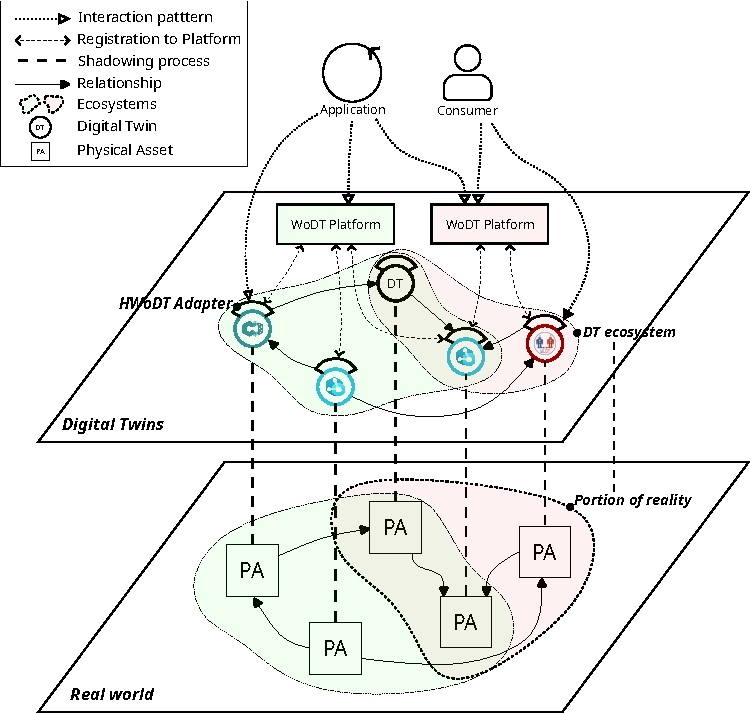
\includegraphics[width=0.65\textwidth]{figures/hwodt/hwodt.pdf}
  \caption{The Hypermedia WoDT scheme, in the real world PAs (squares) belonging to different organizations and domains are connected by relationships. In the digital world, cross-domain ecosystems of DTs (circles) mirror different portions of reality, supported by the WoDT Platform.}
  \label{fig:hwodt}
\end{figure}


\subsection{A Uniform Interface for Heterogeneous \aclp{DT}}\label{ssec:uniform-interface}

As a first step towards integrating heterogeneous \acp{DT} we look into how each individual \ac{DT} can expose a uniform interface, compliant with the requirements of the \ac{HWoDT}.

Achieving standard semantic representations of \acp{DT} is an open challenge for the \ac{DT} community~\cite{burattini2024models}.
In this work, we adopt a pragmatic approach to demonstrate the benefits of uniform semantic representations in building interoperability within the context of the \acp{DTE}.

Our proposal is grounded on the \ac{HATEOAS} principle of the Web architecture:
each \ac{DT} must be able to provide consumers with both data and \emph{affordances} -- i.e., action possibilities -- through hypermedia representations.
We distinguish two logically different representations:
\begin{itemize}
    \item a \emph{\acf{DTD}}, inspired by the \ac{WoT} \acl{TD}, to hold metadata and affordances, enabling consumers to understand the \ac{DT} model, as well as which services the \ac{DT} exposes and how to access them;
    \item a \emph{\acf{DTKG}} representing the live state of the \ac{DT}, semantically encoding domain knowledge and supporting state observation, querying, and discovering relationships between \acp{DT}.
\end{itemize}

We further require each \ac{DT} to comply with a set of standard \emph{interaction patterns} to allow consumers to uniformly obtain and manipulate such representations for all \acp{DT} in the \ac{HWoDT}.

\subsubsection{The \acl{DTD}}

The \ac{DTD} serves the primary purpose of providing management metadata about a \ac{DT}, registering it within the ecosystem and describing the exposed interactions\footnote{Documentation on the structure of the \ac{DTD} schema is available on GitHub \url{https://github.com/Web-of-Digital-Twins/dtd-conceptual-model}}.

A primary concern is \emph{identification} of the \ac{DT} and the associated \ac{PA} to unambiguously distinguish them from other elements of the ecosystem.
While \acp{PA} may use domain-specific identifiers (e.g., a serial number), we identify each \ac{DT} in a \ac{HWoDT} with a persistent, globally unique \ac{URI}.
This ensures identification and accessibility of \acp{DT} as Web resources throughout their whole lifecycle.

Furthermore, to support navigation from a \ac{DT} to the ecosystem it is part of, the \ac{DTD} also links to the \ac{URI} of the ecosystem, which in our implementation points to the \ac{WoDT} platform.

Other relevant metadata in the \ac{DTD} concerns the model used to represent the \ac{PA} at the digital level.
%
For this, we adopt the \ac{WoDT} metamodel -- closely aligned with the  \ac{WoT} \ac{TD} -- to describe the \ac{DT} in terms of which properties, relationships, events, and actions are available to \ac{DT} consumers. 

Finally, the \ac{DTD} presents a description of the \ac{API} that consumers can use to interact with the \ac{DT}, using hypermedia controls to describe protocol bindings for the exposed interaction patterns.
%
The \ac{DTD}, is thus aligned with \ac{REST} principles as it presents both data and controls to consumers using self-descripting messages.

Even if the \ac{DTD} may evolve with new properties or interactions when a \ac{DT} gets updated, it remains mostly static as it describes the \ac{DT}'s identity metadata and software interface, not its real-time state.

\subsubsection{The \acl{DTKG}}

As a \ac{DT} main responsibility is to provide an up-to-date representation of the \ac{PA} state, to complement the \ac{DTD} we introduce the idea of representing the live state of the \ac{DT} with a \ac{DTKG}. 

The \ac{DTKG} hence serves the purpose of, by means of \ac{RDF} triples, representing:
\begin{inlinelist}
    \item current property values;
    \item current relationships with other \acp{DT};
    \item context-dependent available actions.
\end{inlinelist}
Events, generated by the \ac{DT} are excluded as they are by nature non persistent information handled via subscriptions.

By using \ac{RDF}, the \ac{DTKG} can encode information about the \ac{DT}'s state with explicit semantics using domain-specific ontologies to support a common interpretation of \ac{DT} data.
Additionally, following Linked-Data principles, \acp{DT} linking to other \acp{DT} through relationships supports navigating across the ecosystem in a distributed \ac{KG}.

\subsubsection{\acl{DT} Interaction Patterns}

Other than generating the necessary \ac{DTD} and \ac{DTKG} we require each \ac{DT} in a \ac{HWoDT} ecosystem to implement a Web \ac{API} for consumers. This enables direct use by any Web client.

First, the \ac{API} should expose methods to retrieve the two \ac{DT} representations presented above.
%
As the main function of a \ac{DT} is to represent the \ac{PA} state over time, we choose to return the current \emph{snapshot} of the \ac{DTKG} when dereferencing the \ac{URI} which identifies the \ac{DT} with an HTTP GET request.
%
Technically, since a \ac{DT} qualifies as a \emph{non-information resource}\footnote{For a discussion on information vs. non-information resources see \url{https://www.w3.org/TR/cooluris/} and \url{https://lists.w3.org/Archives/Public/www-tag/2005Jun/0039.html}}
we follow the standard Web practice of returning a 303 (See Other) status code with the \textit{Location} HTTP header set to the \ac{URL} of the \ac{DTKG} information resource.

We link instead the \ac{URL} of the \ac{DTD} in an HTTP Link Header with a custom relation type \texttt{dtd} in the response of the \ac{DTKG} GET request.
%
In this way, consumers can follow links between resources and access both \ac{DT} representations with standard Web interactions  (\Cref{fig:sequence-dtddtkg}).

\begin{figure}[t]
    \centering
     \includegraphics[width=0.7\columnwidth]{figures/hwodt/dtddtkg.pdf}
        \caption{Interaction pattern to access the \ac{DTD} and \ac{DTKG}}
        \label{fig:sequence-dtddtkg}
\end{figure}
  

% \begin{figure}[t]
%     \centering
%     \subfigure[]{
%         \includegraphics[width=0.45\columnwidth]{images/dtddtkg.pdf}
%         \label{fig:sequence-dtddtkg}
%     }    
%     \subfigure[]{
%         \includegraphics[width=0.46\columnwidth]{images/dtdactioncrop.pdf}
%         \label{fig:sequence-action}
%     }    
%     \caption{Interaction patterns to (a) access the \ac{DTD} and \ac{DTKG} and (b) invoking available actions on a \ac{DT} through the uniform interface and standard Web patterns}
%     \label{fig:sequence-interactions}
% \end{figure}

Since the \ac{DTKG} evolves over time to reflect the \ac{PA} state, we require \acp{DT} to support a subscription \ac{API} to observe such changes (e.g., via WebSockets, long-polling, or WebSub~\cite{websub}).
%Modeling the \ac{DTKG} as a Web resource also enables basic historicization using protocols like Memento~\cite{rfc7089memento}.

Finally, the \ac{API} may expose \ac{DT} actions invokable by external consumers.
The \ac{DTKG} shows which actions are currently valid, while the \ac{DTD} describes how to request their execution to the \ac{DT}.
Consumers rely on both to interact (\Cref{fig:sequence-action}) and invalid actions should fail (e.g., with HTTP 403), ensuring consistency with the \ac{DT} model.

\begin{figure}[t]
    \centering
    \includegraphics[width=0.7\columnwidth]{figures/hwodt/dtdactioncrop.pdf}
    \caption{Interaction patterns to invoke available actions on a \ac{DT} through the uniform interface.}
    \label{fig:sequence-action}
\end{figure}

\subsection{Ecosystem Services in the HWoDT}
\label{ssec:ecosystem-services}

In our proposal for realizing the \ac{HWoDT} we implement ecosystem functionalities described in \Cref{ssec:operational-definition} through a middleware:
%
the \emph{\ac{WoDT} Platform} aggregates data from registered \acp{DT} and exposes an \ac{API} that consumers can use to manage and interact with the ecosystem as a whole.

\subsubsection{Managing the \acl{HWoDT}}

Our proposal assumes that \acp{DT} are existing, independently running software entities which implement the uniform interface presented in \Cref{ssec:uniform-interface}.
%
Hence, the \ac{DT} creation is handled by developers with their technology of choice, and adding it to an ecosystem is simply a matter of registering it to a \ac{WoDT} Platform. 
%
We thus expect the platform to expose an \ac{API} that managers -- an external service or a \ac{DT} itself -- can use to submit a \ac{DTD} to register a new \ac{DT} to the ecosystem.
The \ac{DTD} is then stored in a registry, which further allows it to be updated or removed if the \ac{DT} leaves the ecosystem.
%
Consumers can also use the registry \ac{API} to discover which \acp{DT} are in the ecosystem and to filter them based on metadata in the \ac{DTD} --- e.g., they can discover if multiple \acp{DT} in the ecosystem model the same \ac{PA} filtering on the \ac{PA} identifier.

These simple operations are sufficient to manage the ecosystem. We use the \ac{DTD} in the registration request as it provides the necessary metadata to assess membership and compliance requirements as well as the \ac{API} description the platform can use to interact with the \ac{DT} upon registration.
% 
Once registered, the platform uses the \ac{API} description within the \ac{DTD} to access and observe the \ac{DTKG}.  
It can also notify successful registration, enabling the \ac{DT} to record the platform \ac{URI} in its list of ecosystems updating its \ac{DTD} accordingly.

\subsubsection{Exploiting the \acl{HWoDT}}

By observing each individual \ac{DTKG}, the platform can cache the latest update and aggregate them to create a global \ac{DTE} \ac{KG} that can be exploited to implement ecosystem-level services for consumers.
%
The \ac{DTD} and \ac{DTKG} of each \ac{DT} are stored within the \ac{KG}, allowing queries to easily retrieve all available information about a \ac{DT}.
%
Each update of a \ac{DTKG} is processed and merged in the global \ac{KG} so that current representation of the whole ecosystem is always available to consumers.

Within the \ac{DTE} \ac{KG} \acp{DT} \acp{URI} are mapped to local \acp{URL} pointing to the cached representation stored by the platform, allowing consumers navigating within the \ac{KG} to interact only with the platform.
%
When dereferencing the \ac{URL} of a \ac{DT} cache, we use an HTTP Link Header with relation type \texttt{original} to provide consumers the means to access the original \ac{DT} directly if needed.

We identify the \ac{DTE} as a non-information resource and assign it a \ac{URI} which, when dereferenced, returns the global \ac{DTE} \ac{KG}\footnote{As the ecosystem \ac{KG} can be very large, returning the whole thing can be impractical. Alternatives include returning a partial representation with links to the \acp{DT} caches}.

Consumers can also \emph{query} the \ac{DTE} \ac{KG} through the \ac{WoDT} platform SPARQL endpoint~\cite{sparqlprotocol}. 
This enables the extraction of selected information from the current state of all \acp{DT} in the ecosystem with a standard query language.

Finally, consumers may want to observe the evolution of the ecosystem \ac{KG}. The platform must then support an \ac{API} to receive subscription requests and send updates to observers.
%
Given the large nature of the \ac{DTE} \ac{KG}, consumers might not be interested in receiving \emph{all} updates. Hence, techniques for \ac{RDF} stream processing~\cite{barbieri2009www} might be more effective to support selective observation.


%======================================================
\section{A Prototype Framework for the \acs{HWoDT}}
\label{sec:hwodt-impl}
%======================================================

To support the prototyping of heterogeneous \acp{DTE} based on the \ac{HWoDT} proposal, we implement a set of tools aimed at integrating existing \ac{DT} technologies.
%
The tools are open source and available on GitHub
\footnote{\url{https://github.com/Web-of-Digital-Twins}}. 

The software distribution includes a prototype \emph{\ac{WoDT} Platform} implementation and \emph{adapters} to implement the \ac{HWoDT} uniform interface for \acp{DT} developed with \azureTwin{}\footnote{\url{https://learn.microsoft.com/en-us/azure/digital-twins/}}, Eclipse Ditto\footnote{\url{https://eclipse.dev/ditto/}}, and the \ac{WLDT} library~\cite{picone2021wldt}\footnote{\url{https://wldt.github.io/}}.
We chose these representative technologies as they differ in terms of functionalities, namely \azureTwin{} is a cloud platform, Ditto is an open-source platform, and \ac{WLDT} allows to develop and deploy \acp{DT} as standalone software processes.
This section presents the overall architecture and its implementation.


\begin{figure}[t]
  \centering
  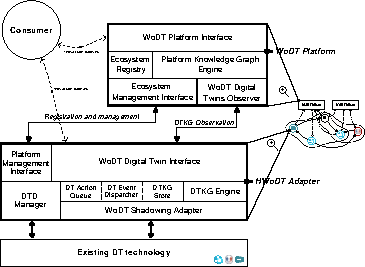
\includegraphics[width=0.65\textwidth]{figures/hwodt/abstract_arch.pdf}
  \caption{Overall abstract architecture of the \ac{HWoDT} framework, showing the main functional modules. On the bottom we have the existing \ac{DT} which, through the adapter, can implement the \ac{HWoDT} uniform interface and be integrated with a \ac{WoDT} platform.}
  \label{fig:abstract_arch}
\end{figure}


\subsection{A \acs{WoT}-compatible \acl{DTD}}

The \ac{DTD} is a central component in the design of the uniform interface of the \ac{HWoDT}.
%
Its design is inspired to the \ac{WoT} \ac{TD}, as an \ac{API} description of the functionalities offered by a \ac{DT}.

Although the \ac{WoT} explicitly reference \acp{DT} in its architectural patterns, the \ac{TD} alone does not support all the metadata that we wish to include in the \ac{DTD}.
Hence, using \ac{WoT}-compliant mechanisms, we extend the \ac{TD} to include the relevant metadata in order to qualify as a functional \ac{DTD} for our prototype implementation of the \ac{HWoDT}.

Namely, we enrich the \ac{TD} using a custom \acl{OWL} \emph{\ac{WoDT} vocabulary}\footnote{\url{https://github.com/Web-of-Digital-Twins/wodt-vocabulary}}
which defines concepts to implement the \ac{DTD} and the \ac{DTKG}, as well as HTTP Link Headers relation types used in the interactions of the \ac{HWoDT} (see \Cref{ssec:uniform-interface}).
%
\Cref{lst:dtd-thing-model} shows a generic \ac{TM}~\cite{wotthing} that can be used to implement a valid \ac{DTD}. We force the \ac{DTD} to include \begin{inlinelist}
    \item the \ac{PA} identifier, 
    \item a link to the \ac{DTKG}, and
    \item an \texttt{observeallproperties} affordance to subscribe to updates of the \ac{DTKG}.
\end{inlinelist} 

\lstinputlisting[
    label={lst:dtd-thing-model},
    caption={The Thing Model that Thing Descriptions must
    implement to be recognized as a valid \acl{DTD}.},
]{listings/hwodt/dtd.jsonld}

The alignment with the \ac{WoT} is strategic for the \ac{DT} community~\cite{etsi2024tr103845,laurinaho2020datalink} as reusing the existing standard ensures compatibility with tools and favors the development of application mashups.

\begin{figure}[t]
  \centering
  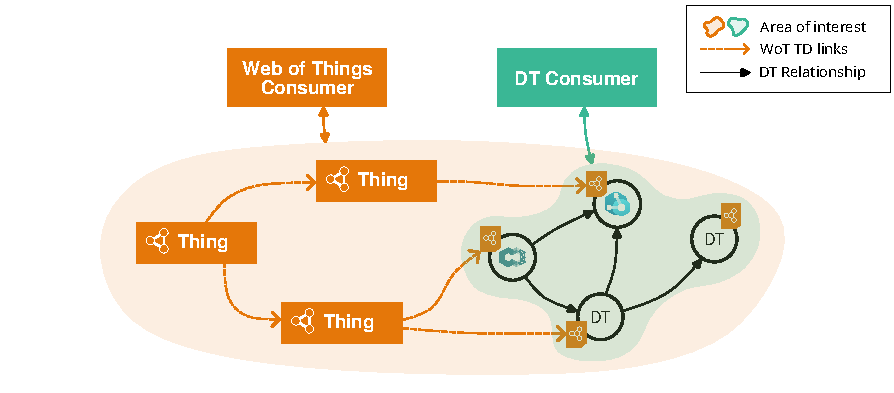
\includegraphics[width=\columnwidth]{figures/hwodt/wot-dt-mashups.pdf}
  \caption{Keeping Digital Twin representations aligned with the \ac{WoT} Thing Description enables the creation of mixed mashups and interoperability with existing \ac{WoT} consumers.}
  \label{fig:wot-dt-mashups}
\end{figure}


\subsection{\acs{DT} Adapters}
\label{ssec:adapters}

\acp{DT} in a \ac{HWoDT} ecosystem must all adhere to the uniform interface, regardless of the technology used to implement them.
%
Adapting existing \ac{DT} technologies to the \ac{HWoDT} interface requires aligning data and interaction patterns.
%
By developing and providing \emph{adapters} for mainstream technologies, we showcase how this alignment can be achieved via configurable reusable components.

This section briefly presents the current adapters developed in the \ac{HWoDT} Framework, following the abstract architecture in \Cref{fig:abstract_arch} (bottom). 
%
We provide adapters for two mainstream platforms (\azureTwin{} and Eclipse Ditto) and the \acl{WLDT} framework, demonstrating the feasibility and supporting the integration of diverse technologies within a \ac{HWoDT} ecosystem.
All adapters support HTTP interactions and WebSocket-based \ac{DTKG} observation.

\subsubsection{\azureTwin{} Adapter}

\azureTwin{} is Microsoft's domain-independent \ac{PaaS} \ac{DT} solution, supporting the management of multiple \acp{DT} connected within a \emph{twin graph}.

Creating \acp{DT} in \azureTwin{} requires defining their model using Azure's \emph{\acf{DTDL}}~\footnote{\url{https://github.com/Azure/opendigitaltwins-dtdl/blob/master/DTDL/v3/DTDL.v3.md}}, a JSON-LD format to specify properties, relationships, commands (actions) and telemetry (events).
%
\ac{DTDL} models can then be used to create \ac{DT} instances.
%
Although the model closely aligns with the \ac{WoDT} model, the support of events and actions is partial\footnote{As of June 2025, commands can be defined but not invoked automatically, while telemetries are not used within \azureTwin{} \url{https://learn.microsoft.com/en-us/azure/digital-twins/concepts-models}} and relationships are limited to linking \acp{DT} within the same \azureTwin{} instance, which hence defines a closed homogeneous ecosystem.

We implement the \azureTwin{} adapter as a middleware, connecting to a \azureTwin{} instance and mapping \acp{DT} to the \ac{HWoDT} uniform interface.
%
The adapter can be configured to select which \acp{DT} needs to be mirrored and specify the mapping from \ac{DTD} properties and relationships to produce the \ac{DTKG}. 
Additionally, the following Azure service pipeline must be set up to link the \azureTwin{} instance to the adapter:
\begin{itemize}
    \item \textit{Azure Event Grid} to capture and forward \azureTwin{} events;
    \item \textit{Azure Function} (\acl{FaaS}) to fetch the current \ac{DT} state and send it to the adapter via SignalR on every new event;
    \item \textit{Azure SignalR} to deliver \acp{DT} state updates to the adapter.
\end{itemize}

The adapter can be deployed either within the Azure cloud or is designed to automatically retrieve the \ac{DTDL} models, stored on \azureTwin{}, and convert them in valid \acp{DTD} for each \ac{DT} instance.
The adapter waits for SignalR events to receive \ac{DT} state updates generated by the Azure Function and convert them into \acp{DTKG} updates.

\subsubsection{Eclipse Ditto Adapter}

\emph{Eclipse Ditto}, is an open-source \ac{DT} platform from the Eclipse Foundation. 
It abstracts each \ac{PA} as a \emph{Ditto Thing} and offers a Web-based layer for interacting with \ac{IoT} devices through their \acp{DT}.

A Ditto instance can manage multiple \acp{DT}, using a metamodel with:
\begin{inlinelist}
    \item \emph{Attributes} for static metadata,
    \item \emph{Features} which can group data (properties) and functionalities (messages).
\end{inlinelist}
Although lacking native support for relationships, actions, and events, these can be modeled using attributes (for links), consumer-to-\ac{DT} messages (for actions), and \ac{DT}-to-consumer messages (for events). Models can be defined via a custom JSON format or a (set of) \ac{WoT} \ac{TM}.

Eclipse Ditto is implemented with a microservice architecture. 
Despite Ditto being open-source and allowing the development of custom extensions, for our prototype we implemented the adapter as a custom external middleware that can be deployed to map one Ditto Thing to the \ac{HWoDT} uniform interface.
%
The middleware leverages Eclipse Ditto’s native WebSocket interface to retrieve data and performs two key transformations: converting the \ac{WoT} \ac{TD} exposed by Ditto into a \ac{DTD}, and serializing \ac{DT} data into a \ac{DTKG}.
This process relies on a configurable mapping between Ditto features and their corresponding \ac{RDF} representations.

\begin{figure}[t]
  \centering
  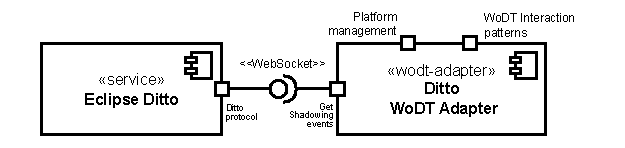
\includegraphics[width=0.8\columnwidth]{figures/hwodt/ditto-adapter-c&c.pdf}
  \caption{The Eclipse Ditto adapter, implemented as a standalone component that maps a specific instance of a \ac{DT} hosted on the Ditto platform.}
  \label{fig:ditto-adapter-c&c}
\end{figure}

\subsubsection{\acl{WLDT} Adapter}

The \emph{\acf{WLDT} framework}~\cite{picone2021wldt} enables the development of \acp{DT} as standalone software components deployable across cloud or edge environments.
Its modular and extensible architecture allows for the easy implementation of \ac{HWoDT}-compliant \acp{DT}.
Specifically, we leverage the concept of \emph{Digital Adapter}, used in the \ac{WLDT} architecture to represent digital interfaces through which the \ac{DT} can expose data for consumers.
%
The framework internal metamodel is already aligned with the \ac{HWoDT}, so no additional effort was required to map concepts.
The adapter is provided as a reusable Java library, which \ac{WLDT} developers can easily import into their projects and use to configure the mapping towards the \ac{HWoDT} uniform interface leveraging the implementation of the necessary \ac{API} to manage the \ac{DTD} and \ac{DTKG}.

\begin{figure}[t]
  \centering
  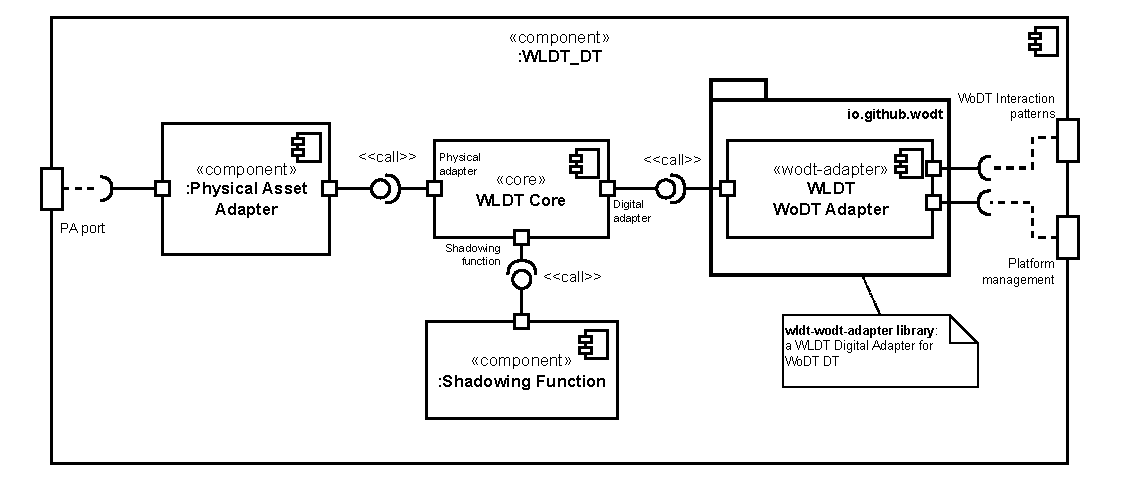
\includegraphics[width=\columnwidth]{figures/hwodt/wldt-adapter-c&c.pdf}
  \caption{The architectural diagram of the \ac{WLDT} adapter, illustrating its integration with the other components of the framework.}
  \label{fig:wldt-adapter-c&c}
\end{figure}

\note{subfigure}
% \begin{figure}[t]
%     \centering
%     \subfigure[]{
%         \includegraphics[width=0.48\textwidth]{figures/hwodt/observation-delay.pdf}
%         \label{fig:observation-delay}
%     }    
%     \subfigure[]{
%         \includegraphics[width=0.48\textwidth]{figures/hwodt/query-delay.pdf}
%         \label{fig:query-delay}
%     }    
%     \caption{Average delay over time with (a) one client observing each \ac{DT} and one observing the Platform \ac{KG} and (b) one client or one client per \ac{DT} performing SPARQL queries every second.
%      Results are plotted with a bucketed average with 3-second intervals, followed by a moving average with a window size of five.}
%     \label{fig:sequence-interactions}
% \end{figure}


\subsubsection{Implementing Custom Adapters}
The description of the adapters implemented in our prototype \ac{HWoDT} framework should be useful for any \ac{DT} developer wishing to implement a custom adapter for their own \ac{DT} or \ac{DT} technology. 
%
The idea of the \ac{HWoDT} is grounded on the fact that implementing such custom adapters is relatively straightforward and that the little effort spent in developing (or even less in configuring) them can bring benefits in the integration with the \ac{HWoDT} ecosystem.
%
We decided to develop adapters for three different \ac{DT} technologies to both support and test heterogeneous \ac{DTE} deployments, but also to demonstrate the feasibility of mapping different models in the \ac{HWoDT} uniform interface.

To summarize, the steps to develop a custom adapter are: 
\begin{inlinelist}
    \item understand how to map the concept of the original \ac{DT} model into the \ac{WoDT} metamodel;
    \item understand how to represent the state of the \ac{DT} with an evolving semantic representation for the \ac{DTKG};
    \item implement a module that can reactively produce the \ac{DTKG} whenever the \ac{DT} state is updated;
    \item implement a module that can serve the \ac{DTD} over HTTP, alongside the mandatory \ac{API} for \ac{DTKG} observation.
\end{inlinelist}

\subsection{The \acs{WoDT} Platform}

We developed a prototype of a \ac{WoDT} Platform in Kotlin, realizing the \ac{HWoDT} interaction patterns described in \Cref{ssec:ecosystem-services}.
The platform implements the modules of the abstract architecture shown in \Cref{fig:abstract_arch}, top.
%
Namely, the platform offers multiple interfaces for consumers: an HTTP \ac{API} for \ac{DTE} management (Ecosystem Management Interface) and one for \ac{KG} access with a SPARQL endpoint for read-only queries, as well as a WebSocket endpoint to observe ecosystem updates (\ac{WoDT} Platform Interface).

The platform can process the \ac{WoT}-based \ac{DTD} described above to register \acp{DT}.
When a registration requested is submitted, the platform: \begin{inlinelist}
    \item locates the \ac{DTKG} observation form (\texttt{observeallproperties}) and starts observing the \ac{DT} for updates;\label{step:observe-dtkg}
    \item notifies the \ac{DT} of successful registration to let it update its \ac{DTD} with the platform URI;\label{step:notification}
    \item maps the \ac{DT} \ac{URI} to a local cache URL;
    \item observes \ac{DTKG} updates and merges them into the \ac{DTE} \ac{KG} stored in memory with Apache Jena.
\end{inlinelist}
%
The current prototype supports the observation of \ac{DTKG} through WebSockets for \ref{step:observe-dtkg} and implements \ref{step:notification} sending a request to a hardcoded \texttt{/platform} HTTP endpoint on the \ac{DT}.

Consumers can interact with the \acp{DTE} through the \ac{WoDT} platform
either through (possibly repeated) SPARQL queries to retrieve the information they need or by observing the whole \ac{KG} through WebSockets.
%
In our prototype, we opted for simplicity pushing to all observers the whole \ac{KG} whenever there is an update so that consumers don't need to have specific update handling logic. 
%
We comment on the practical implications of choosing among these different interactions in the following section. 

% \begin{figure}[t]
%   \centering
%   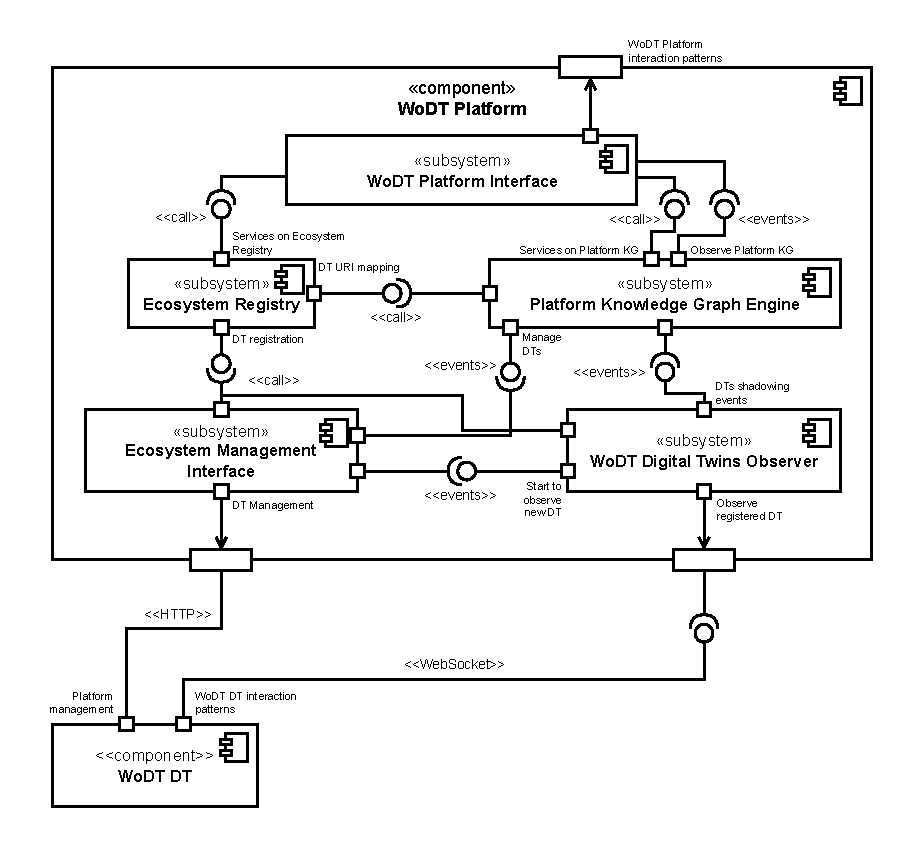
\includegraphics[width=\columnwidth]{images/platform-c&c.pdf}
%   \caption{\ac{WoDT} Platform modules and interfaces, represented using components and connectors.}
%   \label{fig:platform-c&c}
% \end{figure}

\subsection{Prototype Performance Evaluation}
\label{ssec:performance}

\note{TODO: Consider moving this section to the evaluation part}

The primary function of the developed prototype tools is to serve as a reference implementation of the HWoDT proposal, allowing for its value to be shown in practice.
%
Additionally, the prototype has been useful to understand potential performance issues that may arise from applying the adopted architecture, in particular in terms of overhead in the interaction with \acp{DT}.

We focus our evaluation on the \ac{WoDT} platform, as the overhead of adapters is negligible since they perform simple data conversions.
%
We hence design an experiment to stress the performance of the platform in a resource-intensive scenario, and measure the delay perceived by consumers wishing to interact with \acp{DT} and the ecosystem as a whole.

We emulate a \ac{DTE} of a network of temperature sensors \acp{DT} reporting an update every second using \acp{DT} implemented with the \ac{WLDT} framework, running within the same process.
%
Each \ac{DT} generates a random temperature value between 0 and 100 every second, with a random initial offset of up to one second to avoid perfect synchronization.
%
Both the \acp{DT} and the \ac{WoDT} platform run on a single machine equipped with a 13th Gen Intel(R) Core(TM) i7-13700H CPU and 32 GB of RAM, using the OpenJDK 21.0.7 runtime. Platform logs are used to trace and measure delay and we repeat measurements with 50, 100 and 200 \acp{DT} registering data for 10 minutes.

\subsubsection{\acl{KG} Observation}

We measure the average delay in processing an update event from one \ac{DT} with consumers observing each \ac{DT} individually and one observing the whole platform through WebSockets. \Cref{fig:observation-delay} plots average observation latency.
%
As expected, the average delay increases with the number of simultaneously connected DTs. Furthermore, updates on the \ac{DTE} \ac{KG} have a longer delay than updates on individually cached \acp{DTKG}. In our analysis we verified that this is caused by the serialization of the whole KG to stream it at every update, which is computationally intensive. 
%
We can expect the performances to be less drastically impacted when using smarter \ac{KG} update notification strategies -- such as sending incremental changes (e.g., as in \cite{roffia2018fi}) -- at the cost of requiring more complex clients, capable of applying the changes to reconstruct the full state.

% \begin{figure}
%     \centering
%     \includegraphics[width=\columnwidth]{images/observation-delay.pdf}
%     \caption{Average observation delay over time with one client per \ac{DT} and one observing the \ac{DTE} \ac{KG} through WebSockets}
%     \label{fig:observation-dealy}
% \end{figure}

\subsubsection{Repeated Querying}

To evaluate SPARQL query latency, we log the time taken by the platform to handle each request. A lightweight client issues one query per second to retrieve all sensors reporting a temperature above 50 degrees.
%
We test two configurations: one with a single client for the whole platform and another with one client per \ac{DT}.
%
\Cref{fig:query-delay} plots average query latency over time.
%
As expected, query performance is impacted by both the number of \acp{DT}, which increases the size and update rate of the \ac{KG}, and the number of concurrent clients, which increases the platform's load.

\subsubsection{Performance Considerations}

Results indicate that, with a large number of \acp{DT}, using SPARQL queries becomes a more scalable and effective approach for observing the evolution of the ecosystem over time.
%
While this approach may not capture every individual update from each \ac{DT}, it reliably provides the latest available state at the time of each query.
In our experimental setting, for instance, querying every second is realistically sufficient to capture almost all updates, as the client would match the update frequency of the sensors.
This trade-off favors scalability and responsiveness, especially in dynamic settings where maintaining continuous WebSocket subscriptions for all \acp{DT} would be resource-intensive or impractical.
%
Additionally, both figures highlight a cold-start problem caused when all the \acp{DT} register to the platform at the same time. 

% \begin{figure}
%     \centering
%     \includegraphics[width=\columnwidth]{images/query-delay.pdf}
%     \caption{Average query delay over time with either one client per \ac{DT} or just one for the whole \ac{DTE}.}
%     \label{fig:query-dealy}
% \end{figure}


%=======================================================
\section{Semantic Representation for \aclp{DT}}
%=======================================================

\note{Un cappello introduttivo che distingue la proposta del \ac{DTD} + \ac{DTKG} dalle proposte qua sotto}


%\samuele{Discuss the problem of describing a DT in general, possibly presenting a motivating scenario to be used as validation}
In this section, we first define what are the desirable features a DT representation should offer drawing from the conceptual models of DTs and with regard to the problem of interoperability in DT ecosystems that we here summarize as:
\begin{quote}
    Given an ecosystem of DTs we want to allow consumers to easily discover what DTs are present in it, what assets they mirror and how they are mirroring them, the services that the DTs expose and the real-time and past data the DTs are gathering, regardless of the underlying implementing technology.
\end{quote}
We then analyze some notable works in the area to highlight how the idea of introducing a level of representation of DTs is well-recognized in the literature and industry, but at the same time, no existing proposal makes it possible to capture both the structure and the state of a DT in a coherent framework.

\subsection{Requirements for Digital Twins Representations}

When adopting a vision for ecosystems of Digital Twins where several entities of the target domain are digitalized, each through individual DTs, the need to have suitable representations for such DTs emerges quite naturally to achieve several objectives.
This is reflected by DT standardization efforts~\cite{etsi_dt_comm_requirements} that are advocating for descriptions and representations to improve interoperability among different DTs.
%
In this section we will analyze key features that make such a level of representation desirable and will use them as requirements for an ideal representation model for a Digital Twin, to later compare with existing related works.

Two main perspectives are adopted, on one hand, the representation is useful for DT \emph{consumers} i.e., users and application developers that may wish to access the DT data, act on the physical world through the DT or leverage the services offered by the DT. 
On the other hand, the representation can be useful for DT \emph{operators} i.e. DT developers and maintainers that need to manage a complex ecosystem of running instances of DTs, update their models, verify their state of operation and so on.
For both kinds of users, the representations offer a uniform interface to access information about the DT, regardless of the underlying implementing technology.

\paragraph{Identification}
The need to identify uniquely a DT is essential when considering open ecosystems. Moreover, the DT should clearly identify also the unique PA it is representing, as more DTs of the same asset may exist with potentially very different models.

\paragraph{Physical Asset Modelling}
As different DTs for the same asset can be built, the representation of a unique DT should also include information about the models it is offering for the asset. An example of this could be in terms of which properties of the asset are measured and what temporal scale the DT is considered to update their values.
Different models of the same room could very well in fact monitor the current temperature, the average temperature of the last hour or the energy consumption. 

\paragraph{Physical Asset State}
As DT digitalize PAs, one of the core objectives in their representation is making the real-time and past state of the mirrored entity available to consumers.
This allows querying for assets that are in a given state at any given time (e.g. shutting off all devices that are consuming energy over a given threshold).

\paragraph{Service Description}
DTs offer a bi-directional interaction with PAs which allows both to monitor and control the physical reality. Often, their models can also be used to predict or simulate the behaviour of the asset, and in some cases, visualization of the PA state is offered to allow human operators to understand the behaviour of the asset in real time.
In open ecosystems of DTs, all of these features can be exposed as \emph{services} for consumers.
The description of these services is then essential to discovering the capabilities of a DT and using it accordingly, enabling building mashup applications on top of newly discovered DTs, leveraging their services.

\paragraph{Deployment Context}
Technological details concerning how the DT is developed, alongside its version, authors and deployment requirements (e.g. dependency on MQTT brokers, GPU usage) give additional information to system administrators needing to update the DT models, or deploy instances of DTs.
%
Consumers may also choose among different replicas of the same DT the ones that are deployed \emph{closer} to either the source of data or the application depending on their needs.

\paragraph{Metrics and State of Operation}
Metrics concerning its coupling with regard to the PA (e.g. \cite{odte_journal}) allow for assessing the ability of the DT to effectively represent the PA in real time.
Moreover, the lifecycle of a DT can be fairly complex, and a DT could sometimes be disconnected from its physical counterpart. The state of operation of the DT is essential for operators who may need to investigate bugs and consumers who may need to understand that the DT is offline and cannot be used to control the PA.

\paragraph{Data Sources and Storage}
Describing how data is obtained -- i.e., by means of which sources -- allows keeping track of provenance and eases the management of the systems supporting the DT. Additionally, a DT may point to dedicated storage which allows consumers to perform data-intensive operations.
%
%We review the main existing solutions with regard to this requirement to understand whether they suffice already for the goal of supporting interoperable DT Ecosystems.

\subsection{State of the Art Analysis}

\note{FIX TABLE}

% \begin{table*}[ht!]
%     \caption{Surveyed works in the state of the art on DT representations, with the respective features they support: (\checkmark) means the feature is directly supported, ($\sim$) means the feature can be represented within the framework but not explicitly addressed or not completely supported, ($\times$) means the feature is not supported.}  
%     \label{tab:survey}
%     \centering
%     %\renewcommand{\arraystretch}{1}
%     \begin{tabularx}{\textwidth}{X|ccccccc}
%     \toprule
%     \hline
%     \textbf{Representation} & \textbf{Identification} & \textbf{PA Modelling} & \textbf{PA State} & \textbf{Services} & \textbf{Deployment} & \textbf{Metrics} & \textbf{Data} \\
%     \hline
%     \hline
%     Azure DTDL \cite{dtdl} &
%     $\sim$ & 
%     \checkmark &
%     \checkmark &
%     $\times$ &
%     $\times$ &
%     $\sim$ &
%     $\times$  
%     \\
%     \hline
%     WoT Thing Description \cite{wotTD}  &
%     $\sim$ & 
%     \checkmark &
%     $\times$ &
%     \checkmark &
%     $\times$ &
%     $\sim$ &
%     $\times$  
%     \\
%     \hline
%     ETSI SAREF \cite{saref} &
%     $\times$ & 
%     \checkmark &
%     \checkmark &
%     $\sim$ &
%     $\times$ &
%     $\times$ &
%     $\times$  
%     \\
%     \hline
%     Barros et al. \cite{barros2021requirements} &
%     \checkmark & 
%     $\times$ &
%     $\times$ &
%     $\times$ &
%     $\times$ &
%     $\times$ &
%     $\times$ 
%     \\
%     \hline
%     Barth et al.\cite{barth_systematization_2020} &
%     \checkmark & 
%     $\times$ &
%     $\times$ &
%     $\sim$ &
%     $\sim$ &
%     $\times$ &
%     \checkmark  
%     \\
%     \hline
%     Singh et al. \cite{singh_data_2021} &
%     \checkmark & 
%     \checkmark &
%     \checkmark &
%     $\times$ &
%     $\times$ &
%     $\times$ &
%     \checkmark 
%     \\
%     \hline
%     Steinmetz et al. \cite{steinmetz_internet_2018} &
%     \checkmark & 
%     \checkmark &
%     $\times$ &
%     \checkmark &
%     $\times$ &
%     $\times$ &
%     \checkmark 
%     \\
%     \hline
%     Gonzalez et al.\cite{gonzalez-gerpe_wotdt_nodate} &
%     \checkmark & 
%     $\sim$ &
%     $\sim$ &
%     \checkmark &
%     $\times$ &
%     $\times$ &
%     \checkmark 
%     \\
%     \hline
%     \bottomrule
%     \end{tabularx}
% \end{table*}

Having identified the requirements for Digital Twin representations, we believe a complete model should capture all of them in a coherent representation.
%
We then compare relevant works in the state of the art for DT representations with regard to the support of those requirements.
%
We selected them based on their relevance to the topic of creating descriptions for ecosystems of Digital Twins picking from well-known ontologies and data models used in the context of Digital Twins from both industry and academia and selecting among recent works with the keywords ``Digital Twins'' and ``Ontology''. 
%
%Furthermore, to support interoperable ecosystems uniform interfaces are needed to describe DTs with a commonly shared language.
%
%The role of semantics is essential to achieve this, for this reason, we consider mainly models in the state of the art that have explicit semantics and ontologies that have been designed to create representations for Digital Twins.
%
Table~\ref{tab:survey} reports the main analysed works.
%
We do not claim this collection to be exhaustive, but we believe it is a sufficient selection to highlight the open gaps in the area. Additionally, our interest was specifically in works aiming to achieve a description that makes the DT easier to operate with for external consumers. We refer interested readers to a recent survey~\cite{karabulut_ontologies_2024} for a more general analysis of the use of ontologies in Digital Twins.

The Digital Twin Definition Language (DTDL)~\cite{dtdl} is an RDF-based model for the Azure Digital Twins\footnote{\url{https://azure.microsoft.com/en-us/products/digital-twins}} platform by Microsoft.
Its model allows to define models for DTs in terms of their properties, commands and relationships with other twins and to instantiate them within the platform, storing the last updated values of the properties in a so-called \emph{twin graph}.
Even though each instance has an identifier, the represented PA is not identified explicitly.
Azure DT keeps track of the timestamps of the updates of each properties automatically, but does not represent any other metric explicitly, nor it allows to indicate data provenance.

The W3C WoT Thing Description (TD)~\cite{wotTD} is a model to describe connected devices under the abstraction of \emph{things} offering interaction affordances to read properties, execute actions or register to events. A TD identifies ambiguously both a device or a software entity implementing the \emph{thing}---that as per the WoT architecture~\cite{Matsukura:23:WTA} could also be a Digital Twin. Interaction affordances in a TD are equipped with forms to detail how to invoke them, using a specific communication protocol, they thus allow new consumers to understand how to act on the thing and can represent services to interact with the DT.

The Smart Application REference (SAREF) ontology~\cite{saref} by the European Telecommunications Standards Institute (ETSI), is an ontology for IoT applications, that promotes interoperability across several domains. It suits the purpose of representing DTs and a dedicated group is investigating how to adapt it better for the purpose~\cite{etsi_dt_comm_requirements}. SAREF includes concepts such as services, properties and observations to collect the value of specific properties making it a good candidate to represent the model and state of a PA. It is not clear though how it would be possible to identify the software counterpart of the DT, nor how to decorate it with information about the deployment context, metrics or data sources.

Other proposals from the academia~\cite{barth_systematization_2020, barros2021requirements, singh_data_2021, steinmetz_internet_2018} have different objectives with regard to the level of description of a DT. While \cite{barros2021requirements} attempts to link the concept of Digital Twins with foundational ontologies~\cite{guizzardi2022ao} achieving a very high-level description, \cite{barth_systematization_2020} attempts a systematization with respect to the data sources that compose a DT and its value on the target context. Differently \cite{singh_data_2021} and \cite{steinmetz_internet_2018} focus on the IoT domain, with the former focusing on data, whereas the latter focusing on the services and APIs that a DT offers, extending the IoTLite\footnote{\url{https://www.w3.org/submissions//iot-lite/}} ontology to explicitly identify DTs.

A notable work is the recent model proposed by Gonzalez et al.~\cite{gonzalez-gerpe_wotdt_nodate} that extended the WoT TD ontology to represent Digital Twins, explicitly modelling the five-dimensions of DTs~\cite{QI20213}.
With this extension, they can represent the relationship between a DT and its physical counterpart, despite not providing detailed instructions on describing its model or state. Services are represented through TD interaction affordances, and data sources and repositories linked to the DT are represented explicitly through the DCAT\footnote{Data Catalog Vocabulary: \url{https://www.w3.org/TR/vocab-dcat-3/}} ontology, allowing consumers to access also non-semantic data.

% \section{Proposing Semantic Digital Twin Representations}\label{sec:proposal}
% Having identified requirements for interoperability through DT representations that capture the DT structure and state and recognized that existing models generally fall short in representing DTs in their entirety, we here propose an approach based on Linked Data to represent DTs for interoperable ecosystems.

% The approach is based on two main elements: the first is a draft of a core ontology to explicitly identify concepts that are required to represent a DT, the second is an approach to handle browsable DT history using a Linked Data approach.

\subsection{Towards a Core Ontology for Digital Twins}
%\samuele{Present the core model and discuss the main features and motivations}
% \samuele{A diagram of the main entities?}

From the requirements outlined in the previous section, we here sketch a model for a core ontology that can support the definition of DT representations (\Cref{fig:ontology}).
%
Developing an ontology is a long iterative process and as the goal is to support interoperability among the most possible types of DTs we just show here a tentative model that we plan to continue refining in future works.

First, we distinguish clearly the DT from the PA it is mirroring.
Each has a state (and a history, see \cref{ssec:ldp-history}).
The state of the PA includes data about the asset, whereas the state of the DT includes its state of operation, metrics and deployment context.
The DT also has a model, that is described in terms of the features that compose it (properties, actions and events).
Finally, the DT will expose Services, that can be related to other components of the DT -- e.g. the service for subscribing to an event or invoking an action that could be described with a WoT Thing Description~\cite{wotTD} -- or not -- e.g. a simulation service that is generic for the whole DT.

We believe this simple model to be a good start towards the definition of a core ontology, although it will need further refinement and testing with different kinds of DTs.
%
Also, we present this as a core model, since we expect the development of extensions for specific kinds of DTs. Still, having a core root that can already address most requirements can drive interoperability to build DT ecosystems.

\begin{figure}[t]
    \centering
    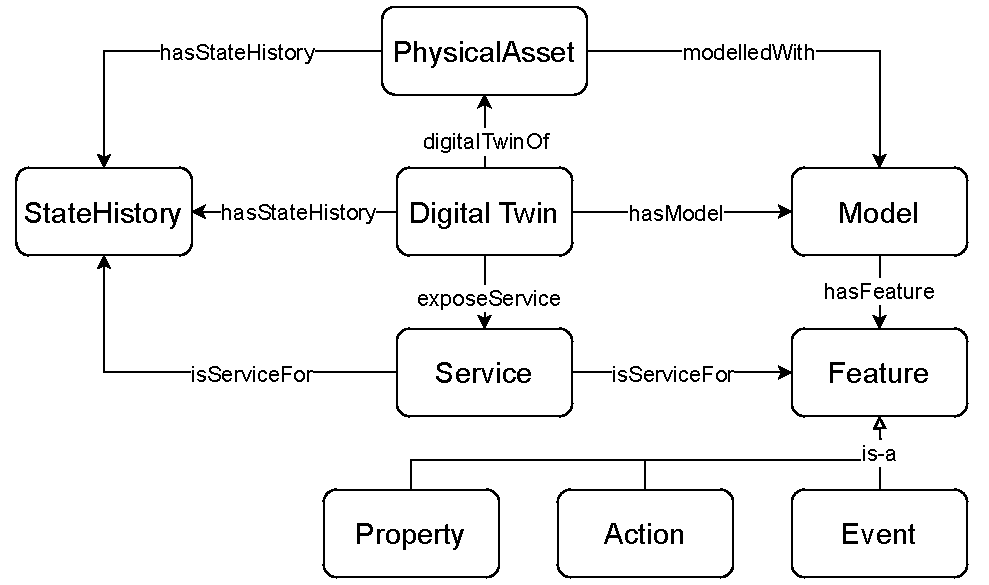
\includegraphics[width=\columnwidth]{figures/edtconf-semantic-rep/ontology.pdf}
    \caption{A schema of the entities for a draft core ontology for DT representations. Relationships are not necessarily 1:1 (i.e., a DT can have multiple Models).}
    \vspace{-1em}
    \label{fig:ontology}
\end{figure}

\subsection{A Linked Data Approach for State History}
\label{ssec:ldp-history}
%\samuele{Discuss the need to store historical version for DTs and the practical alignment with linked data platforms}

Digital Twins by definition evolve over time to reflect the changes of their physical counterparts. As such, their representation must evolve as well. 
%
As can be seen from Table~\ref{tab:survey}, most existing approaches present a level of description that does not include the state of the PA.
%
Nevertheless, this is valuable as it allows clients to directly interrogate the ecosystem of DTs with queries on the current state of a system of DTs.
%
This is supported, for instance, in the Azure Digital Twins platform that offers a representation of a DT in terms of the latest values of its properties, but not its history which is delegated to a separate data storage and as such needs to be accessed with a different tool and query language.

A different approach is instead adopted in other kinds of descriptions such as the one that can be built with the SAREF ontology~\cite{saref} that includes an \texttt{Observation} as a first-class concept to represent the operation that leads to collecting a measurement of some property value at a given time.
%
Managing the evolving state of the asset would then mean adding new observations and property values to the same description. This would make the representation more complete, but also heavier: better for querying but less effective when simply browsing the ecosystem of DTs.

In general, handling the evolution of knowledge graphs over time is a complex subject, but necessary if one wants to keep the representation of a DT up to date.
%
At any given time the representation of the DT should give a consistent and updated representation of its state, while at the same time offering the possibility to browse back in time.
%
For this reason, we envision supporting such a mechanism using the rules of the Linked Data Platform~\cite{Speicher:15:LDP} to host and allow access to the data of a DT.

With every state update, the DT will produce a \emph{snapshot graph} that describes its state at a given time.
%
The DT will then be granted authorized access to POST it as a resource in an LDP Container.
%
If intended as a \emph{named graph}~\cite{Carroll_Bizer_Hayes_Sticker:05} each snapshot of the DT state can further be described in terms of the time frame it represents and with an ordering relationship with the other ones, creating a chain of immutable representations that consumers can browse (Listing~\ref{lst:ldp-history}).
%
The advantage of using the LDP standard would
%make obtaining the representations of the DT state easier for consumers as DTs would
offer a uniform interface for browsing the DT state history.

It must be noted that the semantics of named graphs that we adopted in this paper are still an object of debate in the Semantic Web community\footnote{see \url{https://www.w3.org/TR/2014/NOTE-rdf11-datasets-20140225/} for an in-depth discussion}
% and future interpretations of the concept might require updating this view.
%
We consider this an interesting use case that motivates the need to allow the attribution of names to a graph to further describe it as a whole.

\lstinputlisting[
    float, 
    label={lst:ldp-history}, 
    caption={An example of how the history of the states of the DT can be represented using LDP containers}]
    {listings/edtconf-semantic-rep/ldp-history.ttl}

Of course, this practice is not meant to replace more efficient data storage solutions (e.g. time series databases) that might still be more performing when requiring data in bulk for analytics purposes.
%
This would allow though to have uniform, Linked Data-compliant access to all the features of a DT, enabling browsing through time with pure RESTful interactions. 

% \section{``Validation''}% Demonstrator? Preliminary implementation? Demonstration scenario?
% \samuele{Validate the approach with the scenario, proving that the model is capable of capturing the issues presented in section 3}

\section{Open Challenges and Future Works}\label{sec:challenges}

In this paper, we have outlined the requirements for representations of DTs while showing how existing works fail to capture all of them.
We then suggested how representations based on Linked Data principles can address such requirements:
We advocate for a core ontology for DTs and propose a Linked Data approach to manage DT history under a uniform interface that can be browsed by consumers.

% opennes of the ecosystem vs closed systems (multi-organizations/stakeholders)
% "augmented hardware" and market shares
% distributed nature (linking DTs etc.)
% performance and real-time requirements
% big data storage and retrieval
% Security and access control
% balancing the effort in producing the descriptions for DTs
The vision of interoperable ecosystems of DTs comes with several challenges, both at the technical and societal levels. Here we highlight the main ones and comment on future works.

At the societal level, stakeholders may not be willing to open the data and services of DTs to other consumers, limiting interoperability and preferring the creation of closed systems, especially when DTs are built by companies that sell both the hardware and software counterparts.
%
%The IoT sector has already experienced vendor lock-in and limited interoperability. The proposal of the Web of Things emerged to contrast this providing a shared representation for IoT devices.
%
At the same time, institutions have already shown interest in the realization of DTs for the management of the public infrastructure and open ecosystems of DTs might improve transparency in public settings.
%We believe these players to be the ones that could benefit the most from open interoperable platforms, to improve transparency by producing FAIR\footnote{Findable, Accessible, Interoperable, Reusable} data for the public good~\cite{wilkinson2016fair}.
%
Of course, for this framework to be effective, it must be possible to allow fine-grained access control to data and guarantee security and privacy. We believe the Solid\footnote{\url{https://solidproject.org/}} project to be an interesting direction to achieve this goal in decentralized Linked Data ecosystems.

On the technical level, the main challenges concern the distributed nature of ecosystems of DTs which makes it difficult to create links between DTs, especially when such links are dynamic relationships.  
%
Managing the huge amount of data DTs produce, also challenges the possibility of storing them and interrogating them effectively with knowledge graphs.
%
We believe a hybrid approach to be a plausible solution with DTs' representations pointing to dedicated data storages that use more suitable formats for bulk access.
%
Finally, generating the representations for DTs could be a daunting task for developers, and limit their applicability in practice.
%
We believe development tools should ease this task. A basic core ontology could provide shared structure across different DT development frameworks, leaving only the more domain-oriented aspects to consider for DT developers.

Addressing interoperability is a multi-faceted problem. On one hand, using semantic technologies does not grant interoperability on its own~\cite{guizzardi2020dint} and at the same time, we acknowledge that a core ontology may create a false-agreement problem~\cite{guarino1998formal}. 
%
Nevertheless, this direction can be a step forward:
in future works, we plan to continue developing such core ontology testing the representation of DTs in practical use cases, paired with the Linked Data Platform container approach of \textit{snapshot graphs} for DT history to evaluate its effectiveness.
%
Finally, an essential step will be the creation of alignments with other existing ontologies, to better support representations for DTs across different domains.

